\documentclass[fontsize=26pt,a4paper]{scrartcl}

\usepackage[margin=0.75in,includefoot,bottom=0.3in,footskip=2em]{geometry}

\usepackage{fontspec}
%\setmainfont{EBGaramond}
%[
%  Extension      = .otf,
%  UprightFont    = *-Regular,
%  ItalicFont     = *-Italic,
%  BoldFont       = *-Bold,
%  BoldItalicFont = *-BoldItalic,
%  Numbers        = Lowercase,
%  Ligatures      = Discretionary,
%  Style          = Swash
%]
% https://texnique.fr/osqa/questions/8423/lualatex-et-ligatures

\setmainfont{Palatino Linotype}

\usepackage[french]{babel}
\usepackage{microtype}

%\usepackage{xcolor}
%\usepackage{tikz}
%\usetikzlibrary{intersections,calc}
\usepackage{caption}
\usepackage{longtable,booktabs,array}

\usepackage[showmarks]{pocketmod}% https://github.com/liantze/pocketmod.sty

%\usepackage{graphicx}
\usepackage{enumitem}
\setlist{leftmargin=\parindent,labelindent=*}
\usepackage{hyperref}
\usepackage[hyphenbreaks]{breakurl}

\title{Socrate et la rhétorique}
\author{\small R. Chastain}
\date{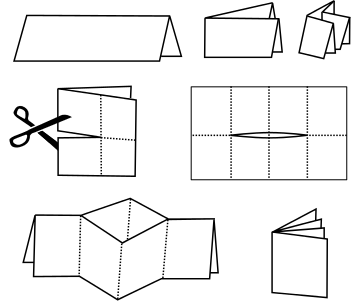
\includegraphics[width=.75\textwidth]{folding-minibook}}

\begin{document}

\thispagestyle{empty}
\maketitle

\clearpage
\subsubsection*{La nature de la rhétorique}

Socrate souhaite savoir quelle est la nature de l'art que Gorgias pratique et enseigne. La rhétorique, répond Gorgias, est l'art de persuader des citoyens réunis en assemblée, au sujet de ce qui est juste. L'orateur n'apporte pas un savoir à ses auditeurs, mais une simple croyance. Pour faire bon usage de son art, il doit avoir la science des choses dont il parle, ou la tenir d'un autre. Il est arrivé à Gorgias d'accompagner un médecin chez un patient qui ne voulait pas se laisser amputer ou cautériser. Tandis que le médecin était impuissant à persuader le patient d'accepter le traitement, Gorgias y parvenait au moyen de l'art oratoire.

Il y a donc un bon et un mauvais usage de la rhétorique. Pour Socrate c'est la preuve que la rhétorique n'est pas un art, car un art a pour objet le bien. La rhétorique n'est qu'un savoir-faire, une habileté à faire plaisir, acquise par expérience.% Ce savoir-faire cependant se fait passer pour un art.

Il existe, pour l'âme comme pour le corps, un état qui s'appelle la santé, et un art qui a pour objet de conserver et de rétablir la santé.% L'art qui a pour objet la santé du corps n'a pas de nom. Ses deux parties sont la gymnastique et la médecine. Quant à l'art qui a pour objet la santé de l'âme, c'est la politique. Les deux parties de la politique sont la législation et la justice.

\begin{longtable}[]{@{}lll@{}}
\toprule()
& Art de conserver & Art de rétablir \\
\midrule()
\endhead Corps & Gymnastique & Médecine \\
Âme & Législation & Justice \\
\bottomrule()
\end{longtable}

Pour chacun de ces arts il existe un savoir-faire qui en est la contrefaçon. La cosmétique, qui donne au corps l'apparence de la santé et de la beauté, contrefait la gymnastique. La cuisine contrefait la médecine. Le cuisinier feint de savoir quels aliments conviennent au corps.% Si un tribunal d'enfants devait décider qui du médecin ou du cuisinier s'y connaît le mieux en nourriture, le cuisinier, s'il le voulait, obtiendrait tous les suffrages.

La législation et la justice ont pour contrefaçon la sophistique et la rhétorique.% Le sophiste contrefait le législateur, comme l'orateur contrefait le juge. La distinction entre sophistique et rhétorique est surtout théorique : dans les faits ce sont souvent les mêmes personnes qui pratiquent l'une et l'autre.

%\begin{longtable}[]{@{}lll@{}}
%\toprule()
%& Faux art de conserver & Faux art de rétablir \\
%\midrule()
%\endhead Santé du corps & Cosmétique & Cuisine \\
%Santé de l'âme & Sophistique & Rhétorique \\
%\bottomrule()
%\end{longtable}

\subsubsection*{Polos ou l'amour du pouvoir}

Les orateurs, objecte Polos, ne sont-ils pas tout-puissants dans la cité ?% Ne peuvent-ils pas faire condamner à mort, à la prison ou à l'exil qui ils veulent ?

Il se peut, répond Socrate, que les orateurs ait le pouvoir de faire tout ce qui leur plaît, mais ils ne font pas pour autant tout ce qu'ils veulent. Ce que nous voulons, dans toutes nos actions, ce n'est pas l'action elle-même, mais sa fin ; et la fin de toutes nos actions est le bien. Par conséquent, celui qui fait \emph{ce qui lui plaît} ne fait pas nécessairement \emph{ce qu'il veut}. L'action qu'il estime avantageuse pour lui peut tourner à son préjudice ; auquel cas il aurait mieux valu pour lui ne pas pouvoir accomplir cette action.% Il est donc clair que cette puissance dont parle Polos, cette liberté de faire ce qui nous plaît, n'est pas un bien en soi : c'est une chose tantôt bonne, tantôt mauvaise. Comment ne pas envier, demande Polos, l'homme qui agit à sa guise dans la cité, qui fait tuer, dépouiller ou jeter en prison qui il lui plaît~?

%\subsubsection*{Le plus grand mal : commettre l'injustice}

D'ailleurs, cet homme, qui fait tuer qui il lui plaît, doit-on supposer qu'il le fait justement ou injustement ? Aux yeux de Polos, la distinction a peu d'importance. Cependant, ni dans un cas ni dans l'autre, dit Socrate, la condition de cet homme n'est enviable. Cet homme est même à prendre en pitié, s'il fait tout cela de manière injuste.% Car le plus grand des maux, c'est de commettre l'injustice.

L'homme le plus malheureux, le plus à plaindre, n'est pas celui qui subit l'injustice, mais celui qui la commet~; et il est plus malheureux encore s'il ne paie point ses fautes et échappe au châtiment qu'il mérite.% Pourtant, ce malheureux parmi les malheureux, c'est celui qu'une part de nous-mêmes envie peut-être en secret ; cette part de nous-mêmes dont Calliclès sera le porte-parole plus loin dans la discussion, lorsque Polos aura à son tour renoncé à tenir tête à Socrate. Pour Polos, l'homme qui est le plus à plaindre, c'est celui qui est victime de l'injustice, celui qu'on fait tuer injustement par exemple. Certes, dit Socrate, c'est un malheur, mais un malheur moins grand 1° que de tuer injustement et 2° que d'être tué justement.

\subsubsection*{Inutilité de la rhétorique}

Le sujet de la discussion est désormais la question de savoir \emph{qui est heureux et qui ne l'est pas}. C'est la question sur laquelle il est le plus beau de savoir la vérité.

Aux yeux de Polos, l'opinion de Socrate est ridicule et facile à réfuter. Socrate prétend au contraire que cette opinion est irréfutable, car c'est, dit-il, la vérité même.% Il y a une opposition diamétrale entre Polos et Socrate, et cette opposition porte à la fois sur la question de savoir qui est heureux ou malheureux, et sur la question de savoir ce qu'est une réfutation.

%Cependant, Socrate et Polos finissent par s'accorder sur un point~: c'est que commettre l'injustice est \emph{plus laid} que de la subir. À partir de ce point concédé par Polos, Socrate montre que commettre l'injustice est aussi plus mauvais. Car ce qui est beau est nécessairement ou agréable ou utile, et inversement ce qui est laid est ou pénible ou nuisible. Or il est moins pénible de commettre l'injustice que de la subir. Il faut donc que ce soit plus mauvais. De même, le juste châtiment que reçoit l'homme qui paie sa faute est beau, quoique pénible~: il est donc bon.

Le criminel qui n'est pas puni pour ses crimes est le plus malheureux des hommes~: il est comme un malade qui ne serait pas soigné. Par conséquent, la rhétorique, qui permet au coupable d'échapper au châtiment, n'a aucune utilité.% À la rigueur, le seul bon usage qu'on pourrait faire de la rhétorique serait de s'accuser soi-même lorsqu'on a commis une faute.

\subsubsection*{Calliclès, ou l'hédonisme radical}

Cette étrange théorie exaspère Calliclès. Socrate plaisante-t-il, ou parle-t-il sérieusement ? S'il est sérieux, et si jamais ce qu'il dit est vrai, alors nous faisons tout le contraire de ce qu'il faudrait.

À en croire Calliclès, il est arrivé à Polos la même chose qu'à Gorgias~: il n'a osé dire ce qu'il pensait. Lorsque Polos a concédé que commettre l'injustice était plus laid que la subir, il a parlé selon la loi, non pas selon la nature. La véritable justice veut que les meilleurs et les plus puissants commandent aux autres et prennent la plus grosse part. Quant à ceux que Socrate appelle les sages, ceux qui se dominent et commandent à leurs passions, ce sont des imbéciles.% Pour être heureux, il faut au contraire, selon Calliclès, entretenir en soi-même les plus fortes passions et leur prodiguer tout ce qu'elles désirent. Le commun des mortels, qui vante la tempérance et la justice, n'est pas sincère~: il ne tient ce discours que pour cacher son impuissance à imiter ceux qu'il envie en secret.

Mais si le bonheur est la même chose que le plaisir, alors avoir la gale et éprouver des démangeaisons continuelles est une vie heureuse, pourvu qu'on ait le pouvoir de se gratter autant qu'on le désire.% Calliclès reproche à Socrate la vulgarité de ses propos. Cependant n'est-ce pas la définition que Calliclès a donnée du bonheur qui a conduit la conversation à ces extrémités~?

En réalité, il est évident que bonheur et plaisir sont deux choses différentes, deux états opposés, comme la santé et la maladie. Le plaisir et la souffrance, au contraire, vont toujours ensemble. Il est agréable de manger quand on a faim, agréable de boire quand on a soif, c'est-à-dire quand on souffre. C'est donc que le plaisir n'est pas le bonheur.% Si le plaisir et le bien sont deux choses différentes, alors l'art et la flatterie sont aussi deux choses différentes, comme Socrate l'avait expliqué à Polos. On peut faire plaisir à quelqu'un sans se soucier de son véritable intérêt. C'est ce que fait souvent le cuisinier~; c'est aussi ce que font souvent le musicien et le poète~: ils ne cherchent qu'à plaire au public, sans s'inquiéter de ce qui est bon pour lui. Or la poésie est une espèce de rhétorique~: le poète fait au théâtre métier d'orateur.

\subsubsection*{Bien employer les jours que nous avons à vivre}

%Face à l'opiniâtreté de Calliclès, Socrate en est réduit à continuer la discussion tout seul.

L'homme tempérant et sage se conduit envers les dieux et envers les hommes de la manière qui convient. Agir comme il convient à l'égard des hommes, c'est être juste. Agir comme il convient à l'égard des dieux, c'est être pieux. L'homme sage ne se laisse détourner de ses devoirs, ni par le plaisir, ni par la peine~: il est donc aussi courageux.

Quant au reproche que Calliclès fait à Socrate, sur son incapacité à se défendre contre l'injustice qu'il pourrait lui arriver de subir, que faut-il en penser~? Si le plus grand mal qui puisse nous arriver était de subir l'injustice, il faudrait avant tout chercher à se rendre fort~: puisque c'est la force qui nous met à l'abri de l'injustice que nous pourrions subir.% Le mieux sera de prendre le pouvoir dans la cité, si possible même un pouvoir tyrannique~; ou au moins d'être l'ami du gouvernement existant. Pour être l'ami du tyran, il faudra lui ressembler, aimer et blâmer les mêmes choses que lui. D'ailleurs, la rhétorique n'est pas le seul art qui nous sauve du péril. La natation, la navigation, la médecine, le font aussi bien. Pourquoi faudrait-il avoir plus de considération pour l'orateur que pour le maître-nageur, le pilote ou le médecin~?

En réalité, la vie, sa durée plus ou moins longue, ne méritent pas de préoccuper un homme vraiment homme~; au lieu de s'attacher à elle avec amour, il faut s'en remettre à la divinité du soin de régler ces choses.% Il faut plutôt se préoccuper de savoir comment nous emploierons les jours que nous avons à vivre. Voulons-nous être bien vu et acquérir du crédit dans la cité~? Il faut nous adapter à la constitution politique du pays dans lequel nous vivions. Si c'est une démocratie, il faudra penser comme le peuple, pour se faire aimer de lui et devenir grand dans la cité. Cependant la véritable tâche de l'homme d'État n'est pas de plaire aux citoyens, mais de faire leur bien, de les rendre meilleurs, c'est-à-dire bons, justes, tempérants, raisonnables. Quant à ce que Calliclès ne cesse de répéter, que Socrate pourrait être injustement accusé et condamné à mort, faute de connaître la rhétorique, Socrate admet qu'une telle chose pourrait bien arriver, et qu'elle n'aurait même rien d'étonnant. En effet, Socrate est l'un des rares Athéniens, pour ne pas dire le seul, qui cultive le véritable art politique. Il ne cherche jamais à plaire par son langage~; il a toujours en vue le bien, et non pas l'agréable. S'il était accusé, il serait comme un médecin traduit devant un tribunal d'enfants par un cuisinier.

\subsubsection*{La mort, le jugement}

La mort n'a rien d'effrayant, pour celui qui n'a aucune faute à se reprocher, ni envers les dieux, ni envers les hommes. Ce qui est vraiment à redouter, c'est d'être coupable au moment de mourir. Socrate propose de raconter une histoire qui le prouve. Calliclès prendra peut-être cette histoire pour un conte~: Socrate, lui, la tient pour vraie.% Aux hommes qui ont mené une existence juste et sainte, il est permis d'aller, après leur mort, dans les îles des Bienheureux, où ils séjournent, à l'abri de tout mal, dans une félicité parfaite. Ceux qui au contraire ont vécu dans l'injustice et dans l'impiété sont envoyés dans un lieu d'expiation et de peine qu'on appelle le Tartare. Autrefois les hommes étaient jugés de leur vivant, le jour de leur mort, par des juges eux-mêmes vivants. Cependant les jugements étaient mal rendus. Aussi Zeus décida-t-il que les hommes seraient jugés après leur mort. Il destina trois de ses fils, Minos, Rhadamanthe et Éaque, à devenir juges après leur mort. Les trois fils de Zeus rendent désormais leur jugement dans une prairie, à un carrefour d'où partent les deux routes qui mènent, l'une aux îles des Bienheureux, l'autre au Tartare. Rhadamanthe juge les hommes de l'Asie, Éaque ceux de l'Europe. Quant à Minos, il a pour fonction de prononcer en dernier ressort, lorsque ses deux frères sont embarrassés. Voilà l'histoire que Socrate a entendu raconter, et qu'il tient pour vraie. La mort~n'est que la séparation de l'âme et du corps. L'âme aussi bien que le corps porte encore, après la mort, les marques que la vie lui a imprimées. Quand le juge examine une âme et qu'il y trouve la marque des iniquités que l'homme a commises de son vivant, il la condamne à être châtiée. Il y a deux sortes de châtiment, l'un qui guérit et l'autre qui sert d'exemple. Ceux qui subissent un châtiment éternel sont le plus souvent des rois ou des hommes puissants. Le reproche que faisait Calliclès à Socrate se retourne contre Calliclès~: il pourrait bien être incapable de de défendre, au moment de comparaître devant Éaque.

\end{document}
